% !TEX program = lualatex
% Source: ../../2025/week8/week8.pdf (20 slides) and week8.ipynb.
\documentclass[12pt,aspectratio=43]{beamer}
% Shared Beamer design. Load after \documentclass using \input.
% Engine: LuaLaTeX. Fonts: UD Digi Kyokasho N (regular/bold), Arial.
\usepackage{luatexja-fontspec}
\setmainjfont[BoldFont={UD Digi Kyokasho N Bold}]{UD Digi Kyokasho N}
\setsansjfont[BoldFont={UD Digi Kyokasho N Bold}]{UD Digi Kyokasho N}
\setmonojfont[BoldFont={UD Digi Kyokasho N Bold}]{UD Digi Kyokasho N}
% Liberation Sans keeps the layout usable on systems without Arial.
\IfFontExistsTF{Arial}{
  \setmainfont{Arial}
  \setsansfont{Arial}
  \setmonofont{Arial}
}{
  \setmainfont{Liberation Sans}
  \setsansfont{Liberation Sans}
  \setmonofont{Liberation Sans}
}
\renewcommand{\kanjifamilydefault}{\gtdefault}

% Typeset mathematics with a dedicated TeX math font, independent of Arial.
\usefonttheme{professionalfonts}
\usepackage[mathrm=sym]{unicode-math}
\setmathfont{Latin Modern Math}
\setoperatorfont{\symup}

\definecolor{courseblue}{HTML}{4472C4}
\definecolor{ruleblue}{HTML}{8FAADC}
\setbeamercolor{normal text}{fg=black,bg=white}
\setbeamercolor{structure}{fg=courseblue}
\setbeamercolor{frametitle}{fg=black,bg=white}
\setbeamercolor{title banner}{fg=white,bg=courseblue}
\setbeamerfont{frametitle}{size=\fontsize{18}{22}\selectfont,series=\mdseries}
\setbeamerfont{quote}{shape=\upshape}
\setbeamersize{text margin left=9mm,text margin right=9mm}
\setbeamertemplate{navigation symbols}{}
\setbeamercolor{page number}{fg=gray,bg=white}
\setbeamertemplate{footline}{%
  \begin{beamercolorbox}[wd=\paperwidth,ht=2.5mm,dp=1.5mm]{page number}
    \hfill{\fontsize{8}{9}\selectfont
      \ifnum\value{framenumber}>0
        \insertframenumber\,/\,\inserttotalframenumber
      \fi}\hspace*{3mm}
  \end{beamercolorbox}}
\setbeamertemplate{headline}{%
  \hfill\textcolor{gray}{\fontsize{6}{7}\selectfont
    \hypersetup{linkcolor=gray}% Keep Beamer's title links in the header color.
    \ifnum\value{framenumber}=0 \insertshortdate\enspace\fi
    \insertshorttitle\space\insertshortsubtitle}\hspace{2mm}\vspace{1.5mm}}
\setbeamertemplate{frametitle}{%
  \vspace{2mm}\centering\insertframetitle\par
  \vspace{-1mm}{\color{ruleblue}\rule{.44\paperwidth}{.5pt}}\par
  \vspace{2mm}}
\setbeamercolor{itemize item}{fg=courseblue}
\setbeamercolor{itemize subitem}{fg=black}
\setbeamercolor{itemize subsubitem}{fg=black}
\setbeamertemplate{itemize item}{\textbullet}
\setbeamertemplate{itemize subitem}{\textnormal{-}}
\setbeamertemplate{itemize subsubitem}{\textnormal{-}}
\setlength{\parskip}{.45em}
\hypersetup{colorlinks=true,urlcolor=courseblue}

% Use \titlepage inside a [t,noframenumbering] frame. The background extends
% 1 mm past both page edges to avoid hairline gaps in PDF viewers.
\setbeamertemplate{title page}{%
  \vspace{2mm}
  \begin{beamercolorbox}[wd=\paperwidth,ht=43mm,dp=13mm,colsep*=1mm,center]{title banner}
    {\fontsize{32}{40}\selectfont\inserttitle\par}
    \vspace{2mm}
    {\fontsize{20}{24}\selectfont\insertsubtitle\par}
  \end{beamercolorbox}
  \vspace{10mm}
  \hfill\insertauthor
}

\graphicspath{{figures/}}
\usepackage{listings}
\usepackage{upquote}
\IfFontExistsTF{Consolas}{\newfontfamily\codefont{Consolas}}{\newfontfamily\codefont{Liberation Mono}}
\definecolor{codevalue}{HTML}{7A3E9D}
\definecolor{codebuiltin}{HTML}{006DB0}
\definecolor{codestring}{HTML}{267348}
\newcommand{\code}[1]{{\codefont #1}}
\lstdefinestyle{python}{
  language=Python,
  basicstyle=\codefont\fontsize{12}{14}\selectfont,
  keywordstyle=\color{codebuiltin},
  keywordstyle=[2]\color{codebuiltin},
  morekeywords=[2]{print,range},
  stringstyle=\color{codestring},
  showstringspaces=false,
  columns=fullflexible,
  keepspaces=true,
  upquote=true,
  tabsize=4,
  breaklines=false,
  backgroundcolor=\color{black!4},
  frame=single,framerule=0pt,framesep=1.7mm,
  xleftmargin=1.7mm,xrightmargin=1.7mm,
  aboveskip=1mm,belowskip=0.5mm,
  literate=*{0}{{{\color{codevalue}0}}}1
    {1}{{{\color{codevalue}1}}}1 {2}{{{\color{codevalue}2}}}1
    {3}{{{\color{codevalue}3}}}1 {4}{{{\color{codevalue}4}}}1
    {5}{{{\color{codevalue}5}}}1 {6}{{{\color{codevalue}6}}}1
    {7}{{{\color{codevalue}7}}}1 {8}{{{\color{codevalue}8}}}1
    {9}{{{\color{codevalue}9}}}1
}
\lstset{style=python}
\setbeamercolor{lesson note}{fg=black,bg=courseblue!9}
\newenvironment{lessonbox}
  {\begin{beamercolorbox}[wd=\linewidth,sep=1.5mm]{lesson note}}
  {\end{beamercolorbox}\par}

\title{計算物理学B}
\subtitle{第八回：モンテカルロ法1}
\author{野垣 康介、藤本 悠輝}
\date{2026/12/8}
\hypersetup{pdftitle={計算物理学B 第八回：モンテカルロ法1},pdfauthor={野垣 康介、藤本 悠輝}}

\begin{document}

\begin{frame}[t,noframenumbering]
  \titlepage
\end{frame}

\begin{frame}{講義予定}
  \setlength{\parskip}{0pt}
  2026年度 第2学期（火曜3限）
  \par\vspace{2mm}
  \begingroup\centering
    \renewcommand{\arraystretch}{1.05}
    \begin{tabular}{@{}l@{\hspace{2mm}}l@{\hspace{4mm}}l@{\hspace{2mm}}l@{}}
      10/6 & 四則演算 & \textcolor{courseblue}{\textbf{12/8}} & \textcolor{courseblue}{\textbf{モンテカルロ1}} \\
      10/27 & 制御文（for, if） & 12/15 & モンテカルロ2 \\
      11/6（金） & 関数 & 12/22 & 微分方程式1 \\
      11/10 & 配列（NumPy） & 1/12 & 微分方程式2 \\
      11/17 & 可視化（matplotlib） & 1/19 & 偏微分方程式1 \\
      11/24 & 数値微分 & 1/26 & 偏微分方程式2 \\
      12/1 & 数値積分 & 2/2 & 根の探索 \\
      \multicolumn{2}{c}{\small ～中間レポート～} & \multicolumn{2}{c}{\small ～期末レポート～}
    \end{tabular}\par
  \endgroup
  \vspace{2mm}
  {\small 10/20は出張で休講。11/6（金）は火曜授業の振替。\par}
  \vspace{1mm}
  {\fontsize{7}{8}\selectfont 日付：\href{https://www.niigata-u.ac.jp/wp-content/uploads/2025/08/schedule_2026.pdf}{令和8年度（2026）新潟大学授業暦}\par}
\end{frame}

\begin{frame}[t]{講義資料とノートブック}
  \begin{itemize}
    \setlength{\itemsep}{3mm}
    \item Google Colab：{\small\url{https://colab.research.google.com/?hl=ja}}
    \item 講義資料：{\small\url{https://github.com/nogaki/Computational_Physics_B}}
    \item 今週の教材：\code{2026/week8/}
    \item スライド：\code{slide.tex}、実習：\code{week8.ipynb}
  \end{itemize}
  \vspace{2mm}
  GitHubからノートブックを開いたら、Colabの「ファイル」から\textbf{ドライブにコピーを保存}します。
\end{frame}

\begin{frame}[t]{今回の内容}
  \begin{itemize}
    \setlength{\itemsep}{3mm}
    \item モンテカルロ積分を期待値として表す
    \item 円の面積から$\pi$を見積もる
    \item 高次元積分と格子法の計算量
    \item メトロポリス法で確率分布を生成する
  \end{itemize}
  \vfill
  \small 乱数を使う数値積分と、確率分布を再現する方法を学びます。
\end{frame}

\begin{frame}[t]{高次元積分と「次元の呪い」}
  \[
    I=\int dx_1\cdots dx_d\,f(x_1,\ldots,x_d)
  \]
  各軸を$n$分割する格子法では、関数評価の回数は
  \[
    N=n^d
  \]
  です。
  \begin{itemize}
    \item 次元$d$が増えると、同じ分割数でも計算点が急増します。
    \item 高次元では、全空間を格子で覆う方法が難しくなります。
  \end{itemize}
  \begin{lessonbox}
    モンテカルロ法は、空間全体の格子を作らず乱数点を標本として使います。
  \end{lessonbox}
\end{frame}

\begin{frame}[t]{1次元積分を期待値に直す}
  区間$[a,b]$で一様分布に従う確率変数$X$の密度は
  \[
    p(x)=\begin{cases}\dfrac{1}{b-a},&a\leq x\leq b,\\0,&\text{otherwise.}\end{cases}
  \]
  したがって
  \[
    I=\int_a^b f(x)\,dx=(b-a)\,\mathbb{E}[f(X)]
  \]
  です。積分を、乱数で得た関数値の平均に置き換えます。
\end{frame}

\begin{frame}[t]{モンテカルロ積分の推定値}
  独立な一様乱数$x_1,\ldots,x_N$を使うと
  \[
    I_N=\frac{b-a}{N}\sum_{i=1}^{N}f(x_i)
  \]
  で積分を近似できます。
  \begin{itemize}
    \item $N$を増やすと、標本平均は期待値に近づきます。
    \item 同じ$N$でも、乱数列が異なれば推定値は変わります。
    \item 誤差の大きさは標本分散から見積もれます。
  \end{itemize}
\end{frame}

\begin{frame}[t]{2次元・高次元への拡張}
  長方形領域$[a,b]\times[c,d]$の面積を$A=(b-a)(d-c)$とすると、
  \[
    I=\int_a^b\int_c^d f(x,y)\,dy\,dx=A\,\mathbb{E}[f(X,Y)]
  \]
  です。独立な一様乱数の点$(x_i,y_i)$から
  \[
    I_N=\frac{A}{N}\sum_{i=1}^{N}f(x_i,y_i)
  \]
  と推定します。積分次元が増えても式は同じ形です。
\end{frame}

\begin{frame}[t]{例：正弦関数の積分}
  正確な値は$\int_0^\pi\sin x\,dx=2$です。一様乱数$X\in[0,\pi]$を使うと
  \[
    I=\pi\,\mathbb{E}[\sin X],\qquad I_N=\frac{1}{N}\sum_{i=1}^{N}\pi\sin x_i
  \]
  \begin{center}
    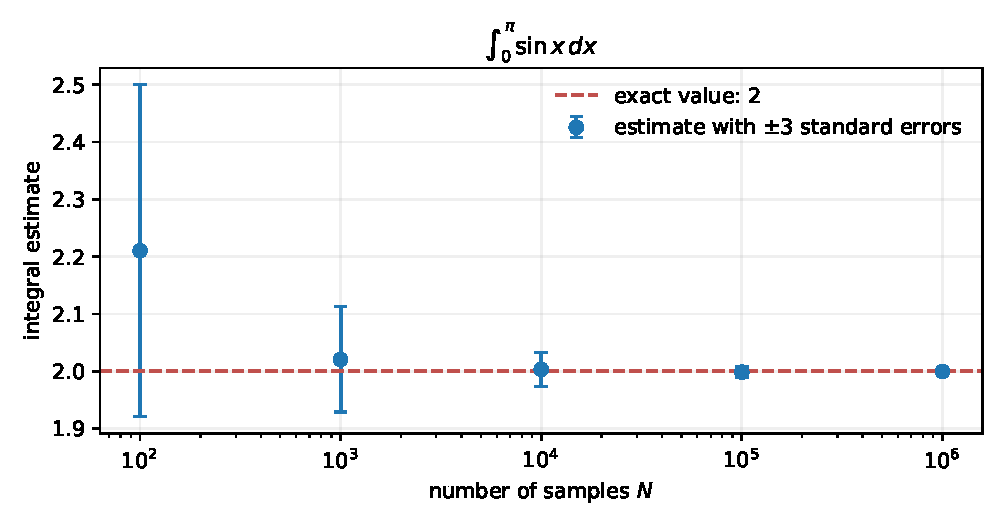
\includegraphics[width=.80\linewidth,height=32mm,keepaspectratio]{sin_monte_carlo.pdf}
  \end{center}
\end{frame}

\begin{frame}[t]{モンテカルロ積分の誤差}
  独立標本で$\operatorname{Var}[f(X)]<\infty$なら、標本平均の標準誤差は
  \[
    \mathrm{SE}(I_N)=\frac{b-a}{\sqrt{N}}\sqrt{\operatorname{Var}[f(X)]}
  \]
  です。中心極限定理により、誤差の代表的な大きさは$O(N^{-1/2})$です。
  \begin{itemize}
    \item 収束次数は積分の次元$d$に直接依存しません。
    \item 係数は関数や次元に依存します。高次元では実用上の誤差が大きくなる場合があります。
  \end{itemize}
\end{frame}

\begin{frame}[t]{格子法との比較}
  $d$次元の各軸を$n$分割し、総点数を$N=n^d$とすると、次数$p$の格子法の誤差は概ね
  \[
    O(n^{-p})=O(N^{-p/d})
  \]
  です。一方、独立標本モンテカルロ法の標準誤差は
  \[
    O(N^{-1/2})
  \]
  です。
  \begin{lessonbox}
    高次元では格子法の収束が遅くなる一方、モンテカルロ法の誤差係数も次元の影響を受けます。
  \end{lessonbox}
\end{frame}

\begin{frame}[t]{円の面積から$\pi$を求める}
  正方形$[0,1]\times[0,1]$に一様乱数点を取ります。
  \[
    p=\Pr(x^2+y^2\leq1)=\frac{\pi}{4}
  \]
  $N$個の点のうち、円内の点が$K$個なら
  \[
    \widehat{\pi}=4\frac{K}{N}
  \]
  と見積もれます。
\end{frame}

\begin{frame}[t]{円内に入る乱数点}
  \begin{center}
    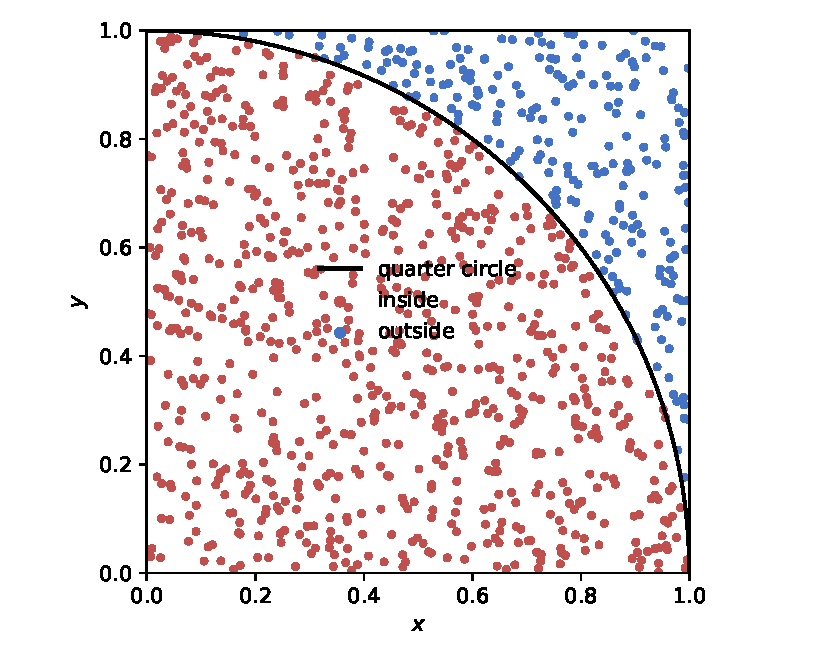
\includegraphics[width=.63\linewidth,height=47mm,keepaspectratio]{circle_points.pdf}
  \end{center}
  \small 赤は円内、青は円外です。点数が少ないと、面積の割合は大きく揺らぎます。
\end{frame}

\begin{frame}[t]{$\pi$の推定誤差}
  独立な一様乱数点を使うと、円内判定は確率$p=\pi/4$のベルヌーイ試行です。
  \[
    \mathrm{SE}(\widehat{\pi})=4\sqrt{\frac{p(1-p)}{N}}
  \]
  \begin{center}
    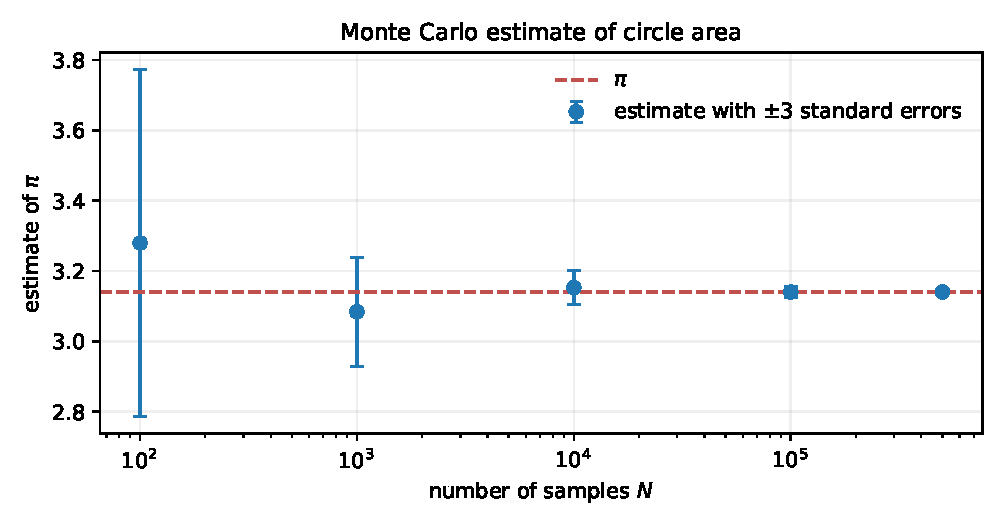
\includegraphics[width=.80\linewidth,height=37mm,keepaspectratio]{pi_convergence.pdf}
  \end{center}
\end{frame}

\begin{frame}[t]{一様乱数が非効率な場合}
  $f(x)$が狭い領域だけで大きい値を取ると、一様乱数ではその領域を十分に訪れないことがあります。
  \[
    \int f(x)\,dx=\int \frac{f(x)}{p(x)}p(x)\,dx
  \]
  \small この書き換えには、$f(x)\ne0$となる領域で$p(x)>0$が必要です。
  \begin{itemize}
    \item 重要な領域で大きい$p(x)$を選ぶ方法を重要度サンプリングと呼びます。
    \item 目的の分布から標本を作る方法の一つがMCMCです。
  \end{itemize}
\end{frame}

\begin{frame}[t]{MCMCで確率分布を再現する}
  目標分布を
  \[
    P(x)=\frac{e^{-S(x)}}{Z},\qquad Z=\int e^{-S(x)}\,dx
  \]
  とします。実際には、規格化定数$Z$が分からず、作用$S(x)$だけが分かる場合もあります。
  \begin{itemize}
    \item 連鎖$x_1\to x_2\to\cdots$を生成します。
    \item 十分長い履歴の頻度で$P(x)$を近似します。
    \item 規格化定数は、遷移確率の比では相殺されます。
  \end{itemize}
\end{frame}

\begin{frame}[t]{マルコフ連鎖の条件}
  \textbf{マルコフ性：}
  \[
    P(x_{k+1}\mid x_k,x_{k-1},\ldots)=P(x_{k+1}\mid x_k)
  \]
  更新は現在の状態だけを使います。
  \begin{itemize}
    \item \textbf{既約性：} 連鎖が可能な状態を行き来できる。
    \item \textbf{非周期性：} 状態への再訪時刻が周期的に固定されない。
  \end{itemize}
  \small 連続状態では、到達可能性は確率密度の台や提案分布で考えます。
\end{frame}

\begin{frame}[t]{詳細つり合い}
  遷移確率$T(x\to x')$が
  \[
    P(x)T(x\to x')=P(x')T(x'\to x)
  \]
  を満たすと、各状態対の確率流がつり合います。
  \begin{itemize}
    \item $P(x)$は連鎖の定常分布になります。
    \item 既約性・非周期性など通常の収束条件のもとで、履歴は目標分布を再現します。
  \end{itemize}
  \small 詳細つり合いは定常分布を作る十分条件の一つです。
\end{frame}

\begin{frame}[t]{メトロポリス法}
  提案分布$q(x'\mid x)$から次の候補$x'$を生成し、確率
  \[
    \alpha(x\to x')=\min\!\left(1,\frac{P(x')q(x\mid x')}{P(x)q(x'\mid x)}\right)
  \]
  で採択します。
  \begin{enumerate}
    \item 候補を提案する。
    \item 0から1の一様乱数と採択確率を比べる。
    \item 採択なら移動し、棄却なら現在の状態に留まる。
  \end{enumerate}
\end{frame}

\begin{frame}[t]{対称な提案分布}
  $q(x'\mid x)=q(x\mid x')$なら、採択確率は
  \[
    \alpha(x\to x')=\min\!\left(1,\frac{P(x')}{P(x)}\right)
  \]
  です。$P(x)\propto e^{-S(x)}$と書けば
  \[
    \alpha(x\to x')=\min\!\left(1,e^{S(x)-S(x')}\right).
  \]
  \begin{itemize}
    \item 目標分布が高い側への提案は必ず採択します。
    \item 低い側への提案も、確率的に採択して探索を続けます。
  \end{itemize}
\end{frame}

\begin{frame}[t]{例：標準正規分布}
  \[
    P(x)=\frac{1}{\sqrt{2\pi}}e^{-x^2/2},\qquad S(x)=\frac{x^2}{2}
  \]
  現在の$x$から、幅$[-1,1]$の一様乱数$\Delta x$を使い
  \[
    x'=x+\Delta x
  \]
  と提案します。初期値を$x=0$として連鎖を進めます。
\end{frame}

\begin{frame}[t]{標本数と分布の再現}
  \begin{center}
    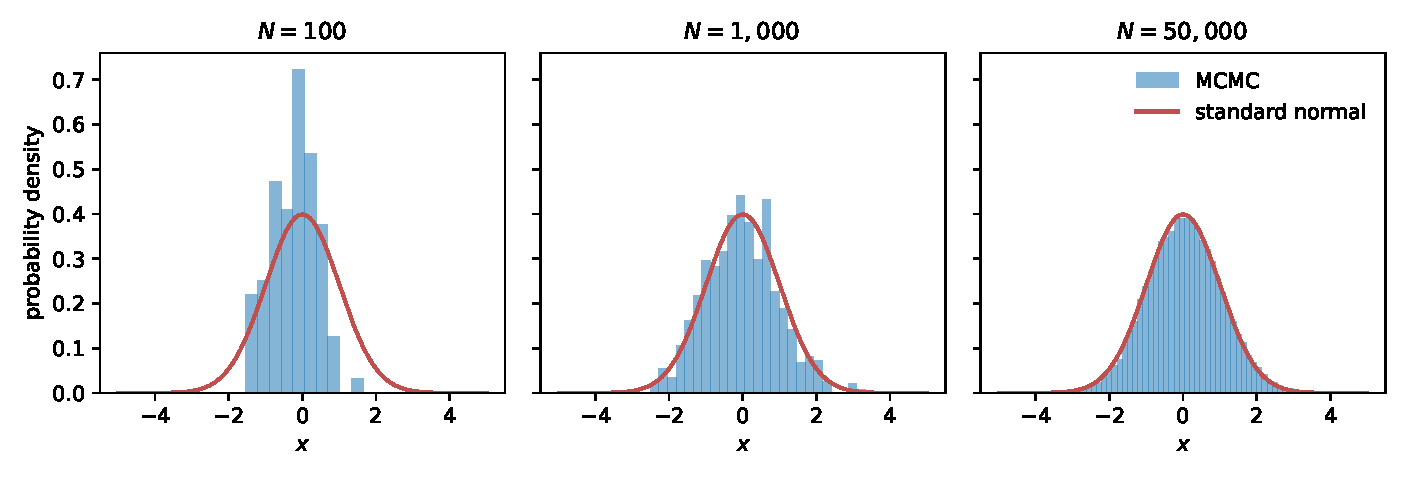
\includegraphics[width=.88\linewidth,height=39mm,keepaspectratio]{metropolis_gaussian.pdf}
  \end{center}
  \small 標本数が増えると、ヒストグラムは標準正規分布に近づきます。再現は有限の標本数で近似的です。
\end{frame}

\begin{frame}[t]{MCMC標本の相関}
  \begin{itemize}
    \setlength{\itemsep}{2mm}
    \item 隣り合う状態は似ていることが多く、標本は独立ではありません。
    \item 正の自己相関では実効標本数が履歴数より小さくなります。
    \item 負の自己相関では$N_{\rm eff}>N$となる場合もあります。
  \end{itemize}
  \[
    N_{\rm eff}\simeq\frac{N}{1+2\sum_{\tau=1}^{\infty}\rho(\tau)}
  \]
  \small 自己相関時間や実効標本数の評価は、次回詳しく扱います。
\end{frame}

\begin{frame}[t]{実習：$d$次元単位球の体積}
  一辺が2の立方体$[-1,1]^d$から点を取り、単位球に入る割合を測ります。
  \[
    \widehat V_d=2^d\frac{K}{N},\qquad
    V_d=\frac{\pi^{d/2}}{\Gamma(d/2+1)}
  \]
  \begin{itemize}
    \item $d=2,4,8$などで推定値と解析解を比べます。
    \item `math.gamma`でガンマ関数を計算できます。
    \item 次元が上がったときの円内・球内の点の割合も調べます。
  \end{itemize}
\end{frame}

\begin{frame}[t]{実習：二峰性分布と疑似乱数}
  \[
    S(x)=-\log\!\left(e^{-\frac12(x-3)^2}+e^{-\frac12(x+3)^2}\right)
  \]
  \begin{itemize}
    \item この作用を持つ確率分布をメトロポリス法で求めます。
    \item 初期値や提案幅を変え、二つの山を探索できるか調べます。
    \item 乱数のシード・周期・統計的性質を調べます。
  \end{itemize}
\end{frame}

\begin{frame}[t]{参考書籍}
  \begin{itemize}
    \setlength{\itemsep}{5mm}
    \item 花田政範・松浦壮『ゼロからできるMCMC：マルコフ連鎖モンテカルロ法の実践的入門』講談社
    \item 野本拓也・是常隆・有田亮太郎『実践計算物理学：物理を理解するためのPython活用法』共立出版
  \end{itemize}
\end{frame}

\begin{frame}[t]{まとめ}
  \begin{itemize}
    \setlength{\itemsep}{3mm}
    \item モンテカルロ積分は、期待値を標本平均で近似します。
    \item 独立標本で分散が有限なら、標準誤差は$O(N^{-1/2})$です。
    \item 高次元での誤差係数や標本の相関は、実際の精度に影響します。
    \item メトロポリス法は、目標分布からの標本列を生成します。
  \end{itemize}
  \vfill
  次回：モンテカルロ法2
\end{frame}

\end{document}
